\section{Inbetriebnahme}



Die Inbetriebnahme der Schaltung erfolgt blockweise. Um gegebenenfalls Fehler in der Schaltung analysieren zu können, werden die einzelnen Schaltungsteile nacheinander aufgebaut und in Betrieb genommen. Die Funktion der zu prüfenden Schaltungsteile wird oberhalb der Tabelle in Stichpunkten erläutert. Bei fehlerhafter Funktion wird diese in der Sektion \glqq Fehleranalyse\grqq{} behandelt.



%%%%%%%%%%%%%%%%%%%%%%%%%%%%%%%%%%%%%%%%%%%%%%%%%%%%%%%%%%%%%%%%%%%%%%%%%%%%%%%%%%%%%%%%%%%%%%%%%%%%%%%%%%%%%%%%%%%%%%%%%																																				%
%														Spannungsversorgung												%
%																														%
%%%%%%%%%%%%%%%%%%%%%%%%%%%%%%%%%%%%%%%%%%%%%%%%%%%%%%%%%%%%%%%%%%%%%%%%%%%%%%%%%%%%%%%%%%%%%%%%%%%%%%%%%%%%%%%%%%%%%%%%%

\subsection{Spannungsversorgung}

%%%%%%%%%%%%%%%%%%%%%%%%%%%%%%%%%%%%%%%%%%%%%%%%%%%%%%%%%%%%%%%%%%%%%%%%%%%%%%%
%																			  %
%								Vorgaben									  %
%																			  %
%%%%%%%%%%%%%%%%%%%%%%%%%%%%%%%%%%%%%%%%%%%%%%%%%%%%%%%%%%%%%%%%%%%%%%%%%%%%%%%

\begin{itemize}
	\item{Spannungen sowie Ströme sind hierbei mit einem Multimeter zu messen.}
	
	\item{Die Funktion der \glqq Meldeleuchte Sicherung\grqq{}  wird durch das Entnehmen der Sicherung aus dem Sockel geprüft. Leuchtet die LED D33 auf, so ist die Funktion dieses Schaltungsteiles gegeben.}
	
	\item{Die Funktion des Verpolungsschutz wird durch das Anlegen einer verpolten Spannung geprüft. Dabei sollte die Strombegrenzung des Labornetzteiles auf ca. 5mA eingestellt sein. Geht das Netzteil bei diesem Test nicht in die Strombegrenzung, so ist die Funktion dieses Schaltungsteiles gegeben.}
\end{itemize}

%%%%%%%%%%%%%%%%%%%%%%%%%%%%%%%%%%%%%%%%%%%%%%%%%%%%%%%%%%%%%%%%%%%%%%%%%%%%%%%
%																			  %
%								Tabelle  									  %
%																			  %
%%%%%%%%%%%%%%%%%%%%%%%%%%%%%%%%%%%%%%%%%%%%%%%%%%%%%%%%%%%%%%%%%%%%%%%%%%%%%%%

\renewcommand{\arraystretch}{2}
\begin{tabularx}{\textwidth}{p{0.2\textwidth}| p{0.6\textwidth} | p{0.05\textwidth} | p{0.1\textwidth}}

 &  & i.o & n.i.o \\

\hline

Stromaufnahme & $I_{G}$: \textcolor{blue}{2,7mA} 			& [x] & [ ] \\

\hline

\multirow{3}{*}{Spannungen}
		& $U_{0}$:   \textcolor{blue}{9,46V}				&	[x] & [ ] 	\\
		& $U_{TP8}$: \textcolor{blue}{9,43V}				&	[x]	& [ ] 	\\
		& $U_{TP9}$: \textcolor{blue}{4,91V}				&	[x] & [ ]  	\\
		
\hline		
		
\multirow{2}{*}{Funktionen}
		& Meldeleuchte Sicherung:  		& [x] & [ ] 	\\
		& Verpolungsschutz:				& [x] & [ ] 	\\ 

\end{tabularx}
\renewcommand{\arraystretch}{1}

\begin{figure}[htb]
    \centering
    \begin{minipage}[t]{0.45\linewidth}
        \centering
        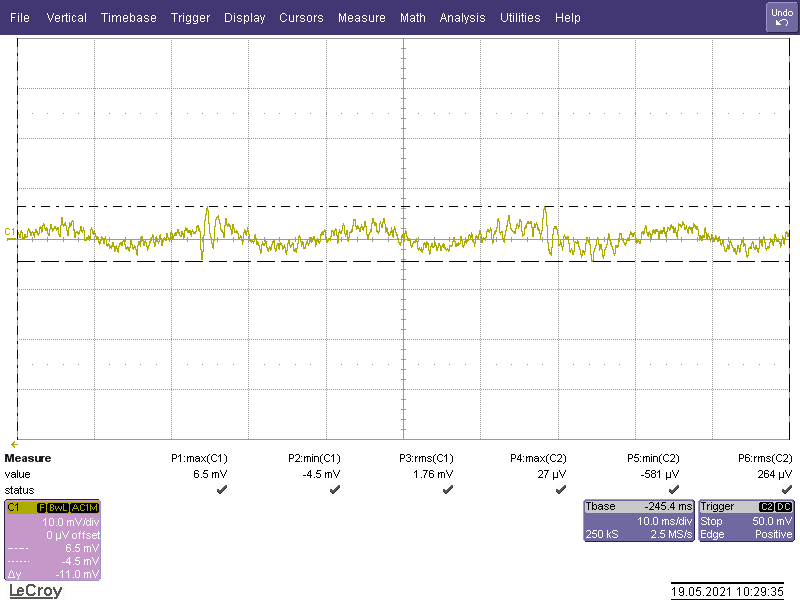
\includegraphics[width=9cm]{Bilder/Versorgungsspannung.png}
        \caption{Versorgungsspannung 5V \\ 11mV Rippelspannung}
    \end{minipage}% <- sonst wird hier ein Leerzeichen eingefügt
   
\end{figure}


%%%%%%%%%%%%%%%%%%%%%%%%%%%%%%%%%%%%%%%%%%%%%%%%%%%%%%%%%%%%%%%%%%%%%%%%%%%%%%%%%%%%%%%%%%%%%%%%%%%%%%%%%%%%%%%%%%%%%%%%%																																				%
%														Taktgeber       												%
%																														%
%%%%%%%%%%%%%%%%%%%%%%%%%%%%%%%%%%%%%%%%%%%%%%%%%%%%%%%%%%%%%%%%%%%%%%%%%%%%%%%%%%%%%%%%%%%%%%%%%%%%%%%%%%%%%%%%%%%%%%%%%

\newpage
\subsection{Taktgeber}

%%%%%%%%%%%%%%%%%%%%%%%%%%%%%%%%%%%%%%%%%%%%%%%%%%%%%%%%%%%%%%%%%%%%%%%%%%%%%%%
%																			  %
%								Vorgaben									  %
%																			  %
%%%%%%%%%%%%%%%%%%%%%%%%%%%%%%%%%%%%%%%%%%%%%%%%%%%%%%%%%%%%%%%%%%%%%%%%%%%%%%%

\begin{itemize}
	\item{Überprüfung der Systemtakte mit Hilfe eines Logikanalysators.}
	
	 \item{Über das Poti soll an TP24 eine Frequenz von 8,5Hz (+-$10\%$) mit einem Tastgrad von 0,5 eingestellt werden.}
	 
	 \item{Durch Betätigen von SW2 kann der Pegel von TP26 gewechselt werden, was durch das optische Signal von D1 oder D2 erkennbar wird.}
	 
	 \item{Die Aufgabe von U14 ist die Signalentprellung des Tasters SW2. Diese Funktion wird durch das oszillieren der Signale U14 Pin 1 und TP25 überprüft. Die Kippzeit des Monoflops soll ca. 500ms betragen.}
	 
	 \item{Leuchtet D2 (Grün), so soll an TP27 die Frequenz von TP24 zu messen sein. Die zu messende Frequenz von TP28 soll dabei die Hälfte von TP27 betragen. Leuchtet D1 (Rot), so soll (sofern kein Verbund aus zwei Messplatinen besteht) keine Frequenz an TP27 und TP28 zu messen sein.}	 
\end{itemize}

%%%%%%%%%%%%%%%%%%%%%%%%%%%%%%%%%%%%%%%%%%%%%%%%%%%%%%%%%%%%%%%%%%%%%%%%%%%%%%%
%																			  %
%								Tabelle  									  %
%																			  %
%%%%%%%%%%%%%%%%%%%%%%%%%%%%%%%%%%%%%%%%%%%%%%%%%%%%%%%%%%%%%%%%%%%%%%%%%%%%%%%

\renewcommand{\arraystretch}{2}
\begin{tabularx}{\textwidth}{p{0.2\textwidth}| p{0.6\textwidth} | p{0.05\textwidth} | p{0.1\textwidth}}

 &  & i.o & n.i.o \\

\hline

Stromaufnahme & $I_{G}$: \textcolor{blue}{6,3mA} & [x] & [ ] \\

\hline

\multirow{2}{*}{Frequenz NE555 }
		& $f_{TP24}$: \textcolor{blue}{8,44Hz}				& [x] & [ ] \\
		& $g_{TP24}$: \textcolor{blue}{0,63}				& [x] & [ ] \\

\hline

\multirow{2}{*}{Taktumschaltung}
		& Taktumschaltung:									&	[x] & [ ] 	\\
		& $t_{Kippzeit}$: \textcolor{blue}{539ms}			&	[x]	& [ ] 	\\
	
\hline		
		
\multirow{3}{*}{Funktionen}
		& Funktion wenn D2 (Grün) leuchtet:  			& [ ] & [x] 	\\
		& $f_{TP28}$: 	\textcolor{blue}{4,23Hz}		& [x] & [ ] 	\\
		& Funktion wenn D1 (ROT) leuchtet:				& [x] & [ ] 	\\ 

\end{tabularx}
\renewcommand{\arraystretch}{1}

\begin{figure}[htb]
    \centering
    \begin{minipage}[t]{0.45\linewidth}
        \centering
        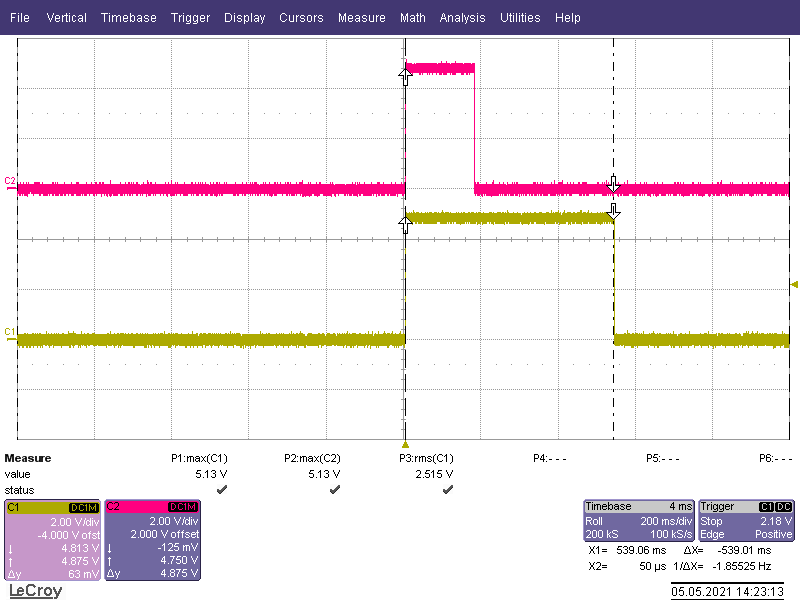
\includegraphics[width=8cm]{Bilder/Kippzeit.png}
        \caption{Kippzeit des Monoflop U14}
    \end{minipage}% <- sonst wird hier ein Leerzeichen eingefügt
       \hfill
    \begin{minipage}[t]{0.45\linewidth}
        \centering
        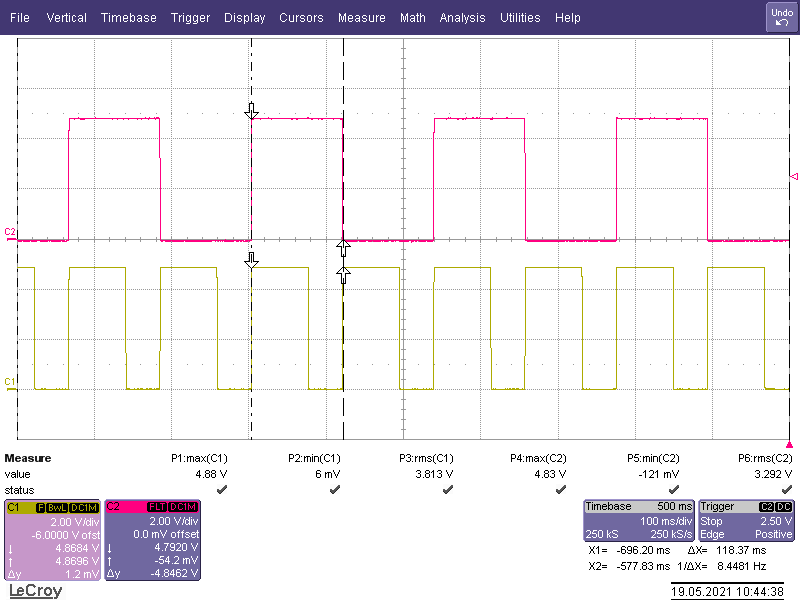
\includegraphics[width=8cm]{Bilder/Systemtakte.png}
        \caption{Teilung des NE555-Takt}
    \end{minipage}
\end{figure}



%%%%%%%%%%%%%%%%%%%%%%%%%%%%%%%%%%%%%%%%%%%%%%%%%%%%%%%%%%%%%%%%%%%%%%%%%%%%%%%%%%%%%%%%%%%%%%%%%%%%%%%%%%%%%%%%%%%%%%%%%																																				%
%														Taktgeber       												%
%																														%
%%%%%%%%%%%%%%%%%%%%%%%%%%%%%%%%%%%%%%%%%%%%%%%%%%%%%%%%%%%%%%%%%%%%%%%%%%%%%%%%%%%%%%%%%%%%%%%%%%%%%%%%%%%%%%%%%%%%%%%%%

\newpage
\subsection{DEZ-Zähler}

%%%%%%%%%%%%%%%%%%%%%%%%%%%%%%%%%%%%%%%%%%%%%%%%%%%%%%%%%%%%%%%%%%%%%%%%%%%%%%%
%																			  %
%								Vorgaben									  %
%																			  %
%%%%%%%%%%%%%%%%%%%%%%%%%%%%%%%%%%%%%%%%%%%%%%%%%%%%%%%%%%%%%%%%%%%%%%%%%%%%%%%

\begin{itemize}
	\item{Wenn die LED D2 (Grün) leuchtet, kann durch Betätigung von SW1 (START)\\ der Messvorgang\\ gestartet werden. Dies macht sich durch das Lauflicht (bestehend aus D39, D40, D41, D42) bemerkbar.}
	
	\item{Nach einer Zeit von ca. 3,6s (Messbar durch Impulszeit von TP20) soll das ganze System durch Betätigung von SW1 erneut gestartet werden können.}
	
	\item{Im Einschaltmoment soll ein verspäteter Nadelimpuls für das korrekte Setzen(default-states) der Schaltung am TP23 gemessen werden können.}
	
	 \item{Leuchtet die LED D1 (Rot), so soll ein Starten der Messung durch Betätigung von SW1 (START) nicht möglich sein.}
\end{itemize}

%%%%%%%%%%%%%%%%%%%%%%%%%%%%%%%%%%%%%%%%%%%%%%%%%%%%%%%%%%%%%%%%%%%%%%%%%%%%%%%
%																			  %
%								Tabelle  									  %
%																			  %
%%%%%%%%%%%%%%%%%%%%%%%%%%%%%%%%%%%%%%%%%%%%%%%%%%%%%%%%%%%%%%%%%%%%%%%%%%%%%%%

\renewcommand{\arraystretch}{2}
\begin{tabularx}{\textwidth}{p{0.2\textwidth}| p{0.6\textwidth} | p{0.05\textwidth} | p{0.1\textwidth}}

 &  & i.o & n.i.o \\

\hline

Stromaufnahme & $I_{G}$: \textcolor{blue}{7,2mA} 					& [x] & [ ] \\

\hline

\multirow{2}{*}{Start Messung}
		& LED D2 und SW1 -> Messung Startet		 					& [x] & [ ] \\
		& $t_{Testzeit}$:	\textcolor{blue}{3,48s}					& [x] & [ ] \\

\hline

\multirow{2}{*}{Nadelimpuls}
		& $t_{Delay}$: \textcolor{blue}{766us}						&[x] & [ ] 	\\
		& $t_{i}$: 	\textcolor{blue}{500us}							&[x] & [ ] 	\\
		
\hline

Tastensperre & LED D1 und SW1 -> Messung Startet nicht 				&[x] & [ ] \\
		
\end{tabularx}
\renewcommand{\arraystretch}{1}

\begin{figure}[htb]
    \centering
    \begin{minipage}[t]{0.45\linewidth}
        \centering
        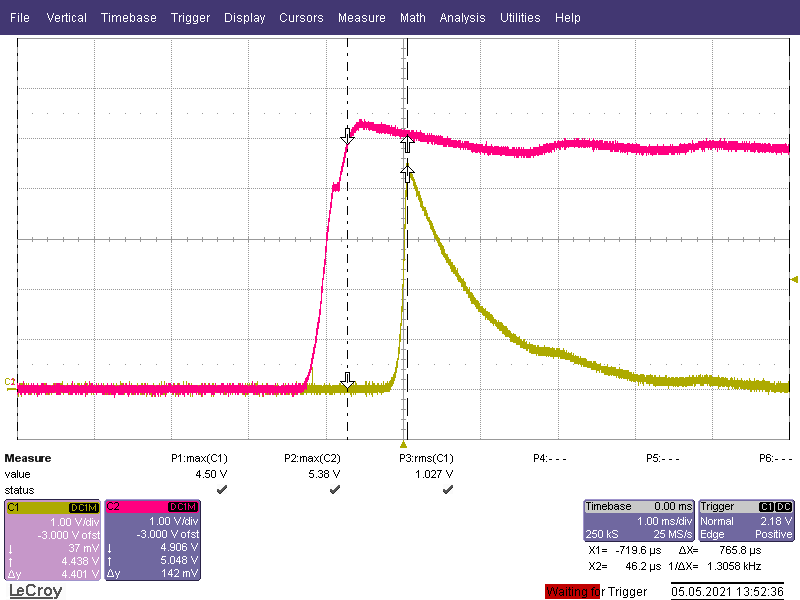
\includegraphics[width=8cm]{Bilder/Resetimpuls.png}
        \caption{Resetimpuls im Einschaltmoment}
    \end{minipage}% <- sonst wird hier ein Leerzeichen eingefügt
    \hfill
    \begin{minipage}[t]{0.45\linewidth}
        \centering
        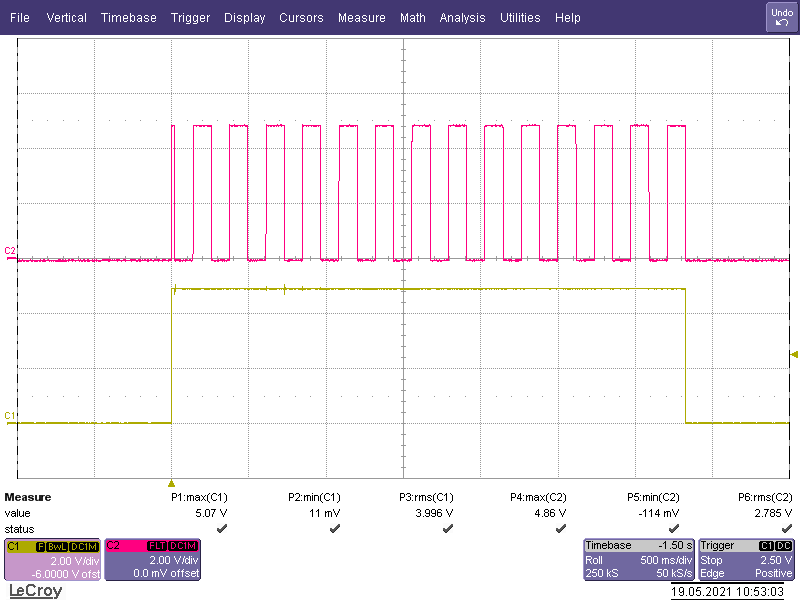
\includegraphics[width=8cm]{Bilder/4Bittakt.png}
        \caption{Taktimpulse nach Starten der Messung}
    \end{minipage} 
\end{figure}

%%%%%%%%%%%%%%%%%%%%%%%%%%%%%%%%%%%%%%%%%%%%%%%%%%%%%%%%%%%%%%%%%%%%%%%%%%%%%%%%%%%%%%%%%%%%%%%%%%%%%%%%%%%%%%%%%%%%%%%%%																																				%
%														Taktgeber       												%
%																														%
%%%%%%%%%%%%%%%%%%%%%%%%%%%%%%%%%%%%%%%%%%%%%%%%%%%%%%%%%%%%%%%%%%%%%%%%%%%%%%%%%%%%%%%%%%%%%%%%%%%%%%%%%%%%%%%%%%%%%%%%%

\newpage
\subsection{Leitungstreiber und Umschaltung}

%%%%%%%%%%%%%%%%%%%%%%%%%%%%%%%%%%%%%%%%%%%%%%%%%%%%%%%%%%%%%%%%%%%%%%%%%%%%%%%
%																			  %
%								Vorgaben									  %
%																			  %
%%%%%%%%%%%%%%%%%%%%%%%%%%%%%%%%%%%%%%%%%%%%%%%%%%%%%%%%%%%%%%%%%%%%%%%%%%%%%%%

\begin{itemize}
	\item{Bei einem High-Signal an TP10 muss das 5V Potenzial auf den Pin 1 von J6 durchgeschaltet werden. Diese Messung muss mit einem Oszilloskop erfolgen, um Pegelschwankungen eindeutig erkennen zu können.}
	
	\item{Nach der Hälfte des High-Signals an TP10 muss auch ein High-Signal an TP11 gemessen werden können.}
	
	\item{Um die Funktion des Analogschalters bestätigen zu können, muss bei gestecktem Jumper (J6) ein 5V Signal für $\dfrac{t_{TP10}}{2}$ an TP5 und TP32 anliegen.}
\end{itemize}

%%%%%%%%%%%%%%%%%%%%%%%%%%%%%%%%%%%%%%%%%%%%%%%%%%%%%%%%%%%%%%%%%%%%%%%%%%%%%%%
%																			  %
%								Tabelle  									  %
%																			  %
%%%%%%%%%%%%%%%%%%%%%%%%%%%%%%%%%%%%%%%%%%%%%%%%%%%%%%%%%%%%%%%%%%%%%%%%%%%%%%%

\renewcommand{\arraystretch}{2}
\begin{tabularx}{\textwidth}{p{0.2\textwidth}| p{0.6\textwidth} | p{0.05\textwidth} | p{0.1\textwidth}}

 &  & i.o & n.i.o \\

\hline

Stromaufnahme & $I_{G}$: \textcolor{blue}{7,6mA} & [x] & [ ] \\

\hline

\multirow{2}{*}{Messspannung}
		& $t_{TP10}$:\textcolor{blue}{228ms}					& [x] & [ ] \\
		& $U_{J6}$: \textcolor{blue}{4,91V}						& [x] & [ ] \\

\hline

\multirow{2}{*}{Umschaltsignal}
		& $t_{delay-TP11}$	\textcolor{blue}{108ms} 				& [x] & [ ] \\
		& $t_{TP11}$: \textcolor{blue}{120ms}						& [x] & [ ] \\

\hline

Umschaltung & Umschaltung von U38A:	& [x] & [ ] \\
		
\end{tabularx}
\renewcommand{\arraystretch}{1}

\begin{figure}[htb]
    \centering
    \begin{minipage}[t]{0.45\linewidth}
        \centering
        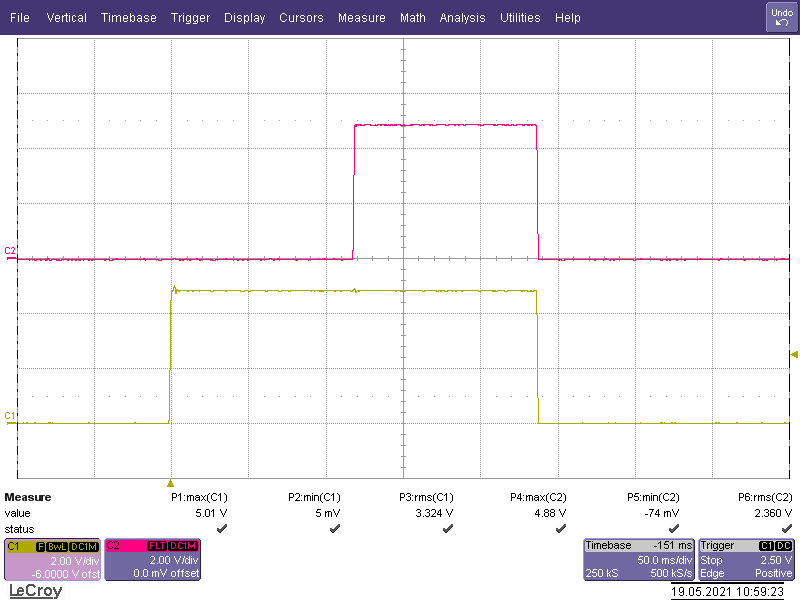
\includegraphics[width=8cm]{Bilder/ASwitch-Umschaltung.png}
        \caption{Umschaltimpuls zwischen den beiden Messungen}
    \end{minipage}% <- sonst wird hier ein Leerzeichen eingefügt
\end{figure}

%%%%%%%%%%%%%%%%%%%%%%%%%%%%%%%%%%%%%%%%%%%%%%%%%%%%%%%%%%%%%%%%%%%%%%%%%%%%%%%%%%%%%%%%%%%%%%%%%%%%%%%%%%%%%%%%%%%%%%%%%																																				%
%														Taktgeber       												%
%																														%
%%%%%%%%%%%%%%%%%%%%%%%%%%%%%%%%%%%%%%%%%%%%%%%%%%%%%%%%%%%%%%%%%%%%%%%%%%%%%%%%%%%%%%%%%%%%%%%%%%%%%%%%%%%%%%%%%%%%%%%%%

\newpage
\subsection{Durchgangsprüfung und Kurzschlussmessung}

%%%%%%%%%%%%%%%%%%%%%%%%%%%%%%%%%%%%%%%%%%%%%%%%%%%%%%%%%%%%%%%%%%%%%%%%%%%%%%%
%																			  %
%								Vorgaben									  %
%																			  %
%%%%%%%%%%%%%%%%%%%%%%%%%%%%%%%%%%%%%%%%%%%%%%%%%%%%%%%%%%%%%%%%%%%%%%%%%%%%%%%

\begin{itemize}
	\item{Analyse des Reset-Impulses, welcher die Schaltung in einen einheitlichen Startzustand bringt.}
	
	\item{Überprüfung der Nadelimpulsunterdrückung durch gleichzeitiges Messen an TP32 und Pin 6 von U30.}
\end{itemize}

%%%%%%%%%%%%%%%%%%%%%%%%%%%%%%%%%%%%%%%%%%%%%%%%%%%%%%%%%%%%%%%%%%%%%%%%%%%%%%%
%																			  %
%								Tabelle  									  %
%																			  %
%%%%%%%%%%%%%%%%%%%%%%%%%%%%%%%%%%%%%%%%%%%%%%%%%%%%%%%%%%%%%%%%%%%%%%%%%%%%%%%

\renewcommand{\arraystretch}{2}
\begin{tabularx}{\textwidth}{p{0.2\textwidth}| p{0.6\textwidth} | p{0.05\textwidth} | p{0.1\textwidth}}

 &  & i.o & n.i.o \\

\hline

Stromaufnahme & $I_{G}$: \textcolor{blue}{7,7mA} 					& [x] & [ ] \\

\hline

Reset-Impuls & $t_{RST}$: \textcolor{blue}{20ns} 					& [x] & [ ] \\

\hline

\multirow{2}{*}{Nadel-Impuls}
		& $t_{TP32_{Nadel-Impuls}}$: \textcolor{blue}{305ns}	 	& [x] & [ ] \\
		& $U_{Pin6 U30_{Nadel-Impuls}}$: \textcolor{blue}{0V}		& [x] & [ ] \\
		
\end{tabularx}
\renewcommand{\arraystretch}{1}

\begin{figure}[htb]
    \centering
    \begin{minipage}[t]{0.45\linewidth}
        \centering
        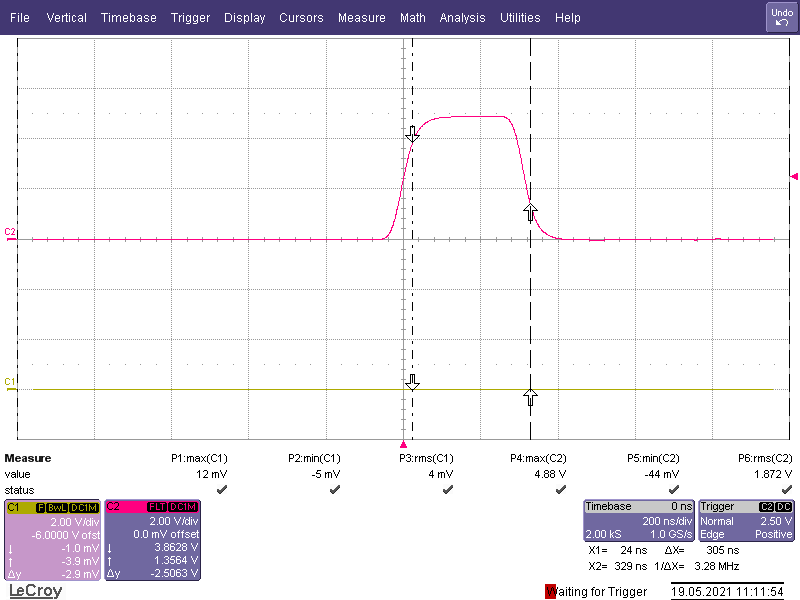
\includegraphics[width=8cm]{Bilder/Fehlerimpuls.png}
        \caption{Unterdrückung eines Set-Impuls im Fehlerfall. }
    \end{minipage}% <- sonst wird hier ein Leerzeichen eingefügt
    \hfill
    \begin{minipage}[t]{0.45\linewidth}
        \centering
        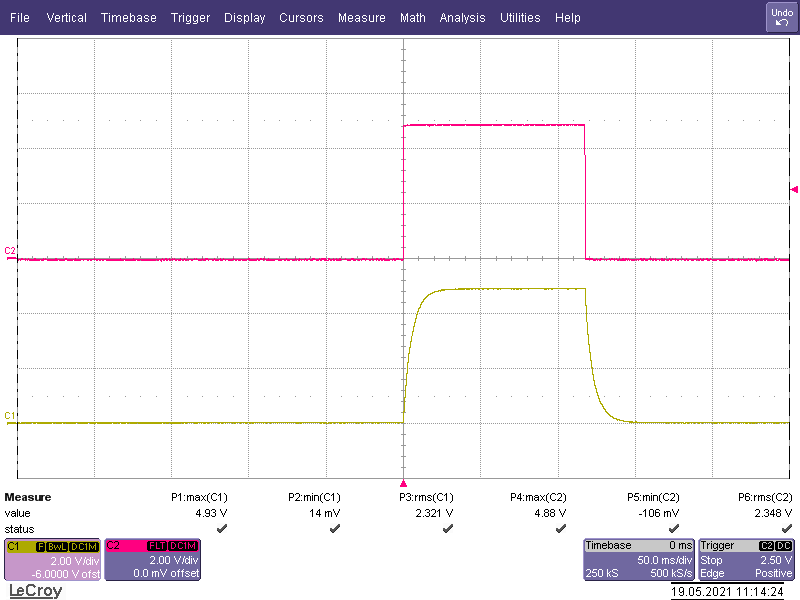
\includegraphics[width=8cm]{Bilder/LowpassFilter.png}
        \caption{Set-Impuls bei fehlerfreier Leitung}
    \end{minipage} 
\end{figure}

%%%%%%%%%%%%%%%%%%%%%%%%%%%%%%%%%%%%%%%%%%%%%%%%%%%%%%%%%%%%%%%%%%%%%%%%%%%%%%%%%%%%%%%%%%%%%%%%%%%%%%%%%%%%%%%%%%%%%%%%%																																				%
%														Taktgeber       												%
%																														%
%%%%%%%%%%%%%%%%%%%%%%%%%%%%%%%%%%%%%%%%%%%%%%%%%%%%%%%%%%%%%%%%%%%%%%%%%%%%%%%%%%%%%%%%%%%%%%%%%%%%%%%%%%%%%%%%%%%%%%%%%

\newpage
\subsection{Konstantstrommessung}

%%%%%%%%%%%%%%%%%%%%%%%%%%%%%%%%%%%%%%%%%%%%%%%%%%%%%%%%%%%%%%%%%%%%%%%%%%%%%%%
%																			  %
%								Vorgaben									  %
%																			  %
%%%%%%%%%%%%%%%%%%%%%%%%%%%%%%%%%%%%%%%%%%%%%%%%%%%%%%%%%%%%%%%%%%%%%%%%%%%%%%%

\begin{itemize}
	\item{Funktion der Konstantstromquelle prüfen durch Stecken eines Jumpers auf J6 und Starten eines Messvorganges. Wenn RV2 und RV3 in Mittelstellung sind, dann ist an TP 6 ein High-Impuls zu erwarten.}
	
	\item{Prüfen, ob die richtigen Takte bzw. Steuersignale an dem Schieberegister anliegen.}
	
	\item{Prüftabelle mit verschiedenen Kabelwiderständen und den dazugehörigen rechnerischen Werten anlegen.}
\end{itemize}

%%%%%%%%%%%%%%%%%%%%%%%%%%%%%%%%%%%%%%%%%%%%%%%%%%%%%%%%%%%%%%%%%%%%%%%%%%%%%%%
%																			  %
%								Tabelle  									  %
%																			  %
%%%%%%%%%%%%%%%%%%%%%%%%%%%%%%%%%%%%%%%%%%%%%%%%%%%%%%%%%%%%%%%%%%%%%%%%%%%%%%%

\renewcommand{\arraystretch}{2}
\begin{tabularx}{\textwidth}{p{0.25\textwidth}| p{0.55\textwidth} | p{0.05\textwidth} | p{0.1\textwidth}}

 &  & i.o & n.i.o \\

\hline

Stromaufnahme & $I_{G}$: \textcolor{blue}{7,9mA} & [x] & [ ] \\

\hline

Konstantstromquelle & Funktion der Konstantstromquelle: 	& [ ] & [x] \\

\hline

Schieberegister Takte & Funktion der Steuersignale: 		& [ ] & [x] \\
		
\end{tabularx}
\renewcommand{\arraystretch}{1}

\vspace{1,5cm}
\textbf{Bemerkung:}
\\
Die Inbetriebnahme dieses Schaltungsteiles hat auf Grund von verschiedenen Fehler einen größeren Zeitraum als geplant eingenommen. Im Kapitel Fehleranalyse wird zwar auf die Fehler und deren Behebung eingegangen, aus zeitlichen Gründen ist dieser Teil aber kein offizieller Teil meines betrieblichen Auftrages.


\begin{figure}[htb]
    \centering
    \begin{minipage}[t]{0.45\linewidth}
        \centering
        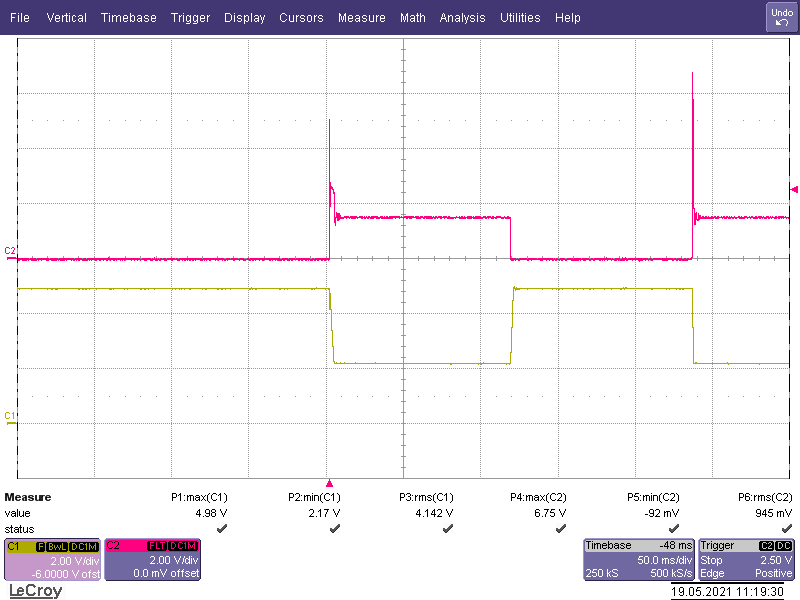
\includegraphics[width=8cm]{Bilder/INA-Spannung.png}
        \caption{CH2 = Spannung nach dem INA (Strommessung)\\
        			CH1 = Regelung des Stromes über die Gate-Source-Spannung}
    \end{minipage}% <- sonst wird hier ein Leerzeichen eingefügt
    \hfill
    \begin{minipage}[t]{0.45\linewidth}
        \centering
        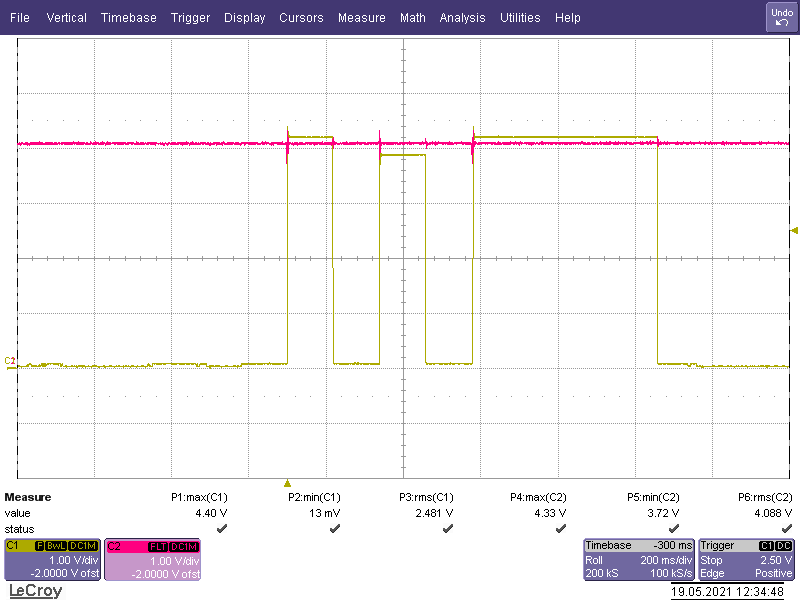
\includegraphics[width=8cm]{Bilder/Auswertung-Widerstand.png}
        \caption{CH2 = Grenzwiderstand (Referenzspannung)\\ 
        			CH1 = Indirekte Widerstandswerte (Spannung über Q1)}
    \end{minipage} 
\end{figure}

Die Abbildung 12 zeigt eine Konstantstrommessung mit 0R, 10R und einem Kurzschluss (von links nach rechts). 

